\documentclass[17pt]{beamer} %Makes presentation
%\documentclass[handout]{beamer} %Makes Handouts
\usetheme{Singapore} %Gray with fade at top
\useoutertheme[subsection=false]{miniframes} %Supppress subsection in header
\useinnertheme{rectangles} %Itemize/Enumerate boxes
\usecolortheme{seagull} %Color theme
\usecolortheme{rose} %Inner color theme

\definecolor{light-gray}{gray}{0.75}
\definecolor{dark-gray}{gray}{0.55}
\setbeamercolor{item}{fg=light-gray}
\setbeamercolor{enumerate item}{fg=dark-gray}

\setbeamertemplate{navigation symbols}{}
%\setbeamertemplate{mini frames}[default]
%\setbeamercovered{dynamics}
\setbeamerfont*{title}{size=\Large,series=\bfseries}
\setbeamerfont{footnote}{size=\tiny}

%\setbeameroption{notes on second screen} %Dual-Screen Notes
%\setbeameroption{show only notes} %Notes Output

\setbeamertemplate{frametitle}{\vspace{.5em}\bfseries\insertframetitle}
\newcommand{\heading}[1]{\noindent \textbf{#1}\\ \vspace{1em}}

\usepackage{bbding,color,multirow,times,ccaption,tabularx,graphicx,verbatim,booktabs}
\usepackage{colortbl} %Table overlays
\usepackage[english]{babel}
%\usepackage[latin1]{inputenc}
%\usepackage[T1]{fontenc}
\usepackage{lmodern}

%\author[]{Thomas J. Leeper}
\institute[]{
  \inst{}%
  Department of Government\\London School of Economics and Political Science
}

\usepackage{tikz}
\usetikzlibrary{shapes,arrows}
\usepackage[normalem]{ulem}

\title{Participant Observation}

\date[]{}

\begin{document}

\frame{\titlepage}

\frame{\tableofcontents}

\section{Interviewing, Continued}
\frame{\tableofcontents[currentsection]}



\frame{
\frametitle{{\normalsize Evaluating a questionnaire}}

\vspace{-1em}

\small

\begin{itemize}\itemsep-0.25em
	\item Is the question easy for respondents to understand?
	\item Are the number and types of response options appropriate?
	\item Are the categories sufficiently distinct from one another?
	\item Is a ``no opinion,'' ``don't know,'' or ``neither support nor oppose'' response option available?
	\item Is one survey item (i.e., one question) sufficient to measure this construct?
	\item How long does it take to read and answer this question?
\end{itemize}
}

\frame{

\frametitle{{\normalsize Cognitive interviewing methods}}

\vspace{-1em}

\small

\begin{itemize}\itemsep-0.25em
\item Retrospective think-alouds (in which respondents describe how they arrive at their answers either just after they provide them or at the end of the interview)
\item Paraphrasing (in which respondents restate the question in their own words)
\item Definitions (in which respondents provide definitions for the key terms in the question)
\item Probes (in which respondents answer follow-up questions designed to reveal their response strategies)
\end{itemize}

}


\frame{
	\frametitle{Problem Set 5}
	\begin{itemize}\itemsep1em
	\item Any questions about Problem Set 5?
	\end{itemize}
}




\section{Participant Observation}
\frame{\tableofcontents[currentsection]}


% activity, thinking about class as a venue





\section{Using Data}
\frame{\tableofcontents[currentsection]}

% something about how to use data gathered from text analysis, interviewing, and participant observation to answer research questions

\frame{

\begin{center}
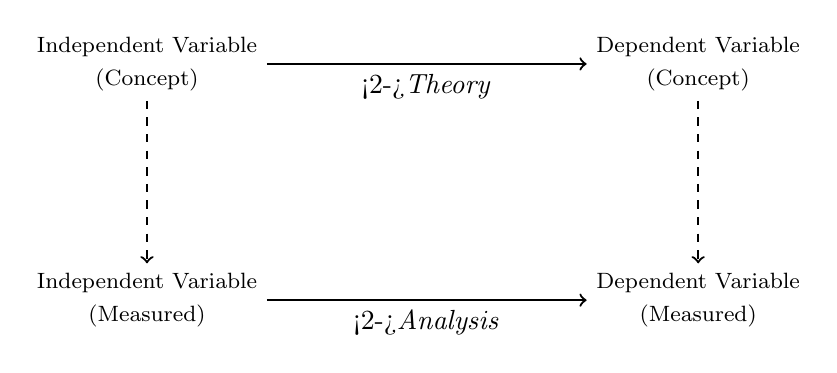
\begin{tikzpicture}
\node [align=center] (ivm) at (0,0) {\footnotesize Independent Variable\\\footnotesize (Measured)};
\node [align=center] (dvm) at (7,0) {\footnotesize Dependent Variable\\\footnotesize (Measured)};

\node [align=center] (ivc) at (0,3) {\footnotesize Independent Variable\\\footnotesize (Concept)};
\node [align=center] (dvc) at (7,3) {\footnotesize Dependent Variable\\\footnotesize (Concept)};

\node (analysis) at (3.5, 0) {};
\node (theory) at (3.5, 3) {};

\draw [->, thick] (ivm) -- (dvm) node[midway, below] (analysis) {{\only<2->{\textit{Analysis}}}};
\draw [->, thick] (ivc) -- (dvc) node[midway, below] (theory) {{\only<2->{\textit{Theory}}}};
\draw [->, dashed, thick] (ivc) -- (ivm);
\draw [->, dashed, thick] (dvc) -- (dvm);
\end{tikzpicture}
\end{center}


}

\frametitle{Operationalization}

\vspace{-2em}

\begin{center}
\tikzstyle{block} = [rectangle, draw, fill=blue!20!white, text width=5em, text centered, rounded corners, minimum height=1em, node distance=7em]
\begin{tikzpicture}[scale=0.5]
\draw<1-> [block] node at (0,0) (concept) {{\Large Concept}};
\draw<1-> [block] node at (-5, -3) (a1) {Attribute};
\draw<1-> [block] node at (0, -3) (a2) {Attribute};
\draw<1-> [block] node at (5, -3) (a3) {Attribute};
\draw<1-> [->, very thick] (concept) -- (a1);
\draw<1-> [->, very thick] (concept) -- (a2);
\draw<1-> [->, very thick] (concept) -- (a3);

\draw<1-> [block, align=center] node at (-11.5, -1.5) (def) {Concept Definition};
\draw<1-> [decorate,very thick, decoration={brace,amplitude=10pt},xshift=-10pt,yshift=0pt]
(-7.5,-3.4) -- (-7.5,0.5);

\draw<2-> [block] node at (-5, -8) (m1) {{\small Measure(s)}};
\draw<2-> [block] node at (0, -8) (m2) {{\small Measure(s)}};
\draw<2-> [block] node at (5, -8) (m3) {{\small Measure(s)}};

\draw<2-> [->, very thick] (a1) -- (m1);
\draw<2-> [->, very thick] (a2) -- (m2);
\draw<2-> [->, very thick] (a3) -- (m3);

\draw<2-> [block, align=center] node at (-11.5, -6.5) (def) {Operation-alization};
\draw<2-> [decorate,very thick, decoration={brace,amplitude=10pt},xshift=-10pt,yshift=0pt]
(-7.5,-8.5) -- (-7.5,-3.6);


\end{tikzpicture}
\end{center}


}





\frame{}


\appendix
\frame{}

\end{document}
